
\documentclass[a4paper,11pt]{article}
\usepackage[a4paper, margin=8em]{geometry}

% usa i pacchetti per la scrittura in italiano
\usepackage[french,italian]{babel}
\usepackage[T1]{fontenc}
\usepackage[utf8]{inputenc}
\frenchspacing 

% usa i pacchetti per la formattazione matematica
\usepackage{amsmath, amssymb, amsthm, amsfonts}

% usa altri pacchetti
\usepackage{gensymb}
\usepackage{hyperref}
\usepackage{standalone}

\usepackage{colortbl}

\usepackage{xstring}
\usepackage{karnaugh-map}

% imposta il titolo
\title{Appunti Calcolatori Elettronici}
\author{Luca Seggiani}
\date{2025}

% imposta lo stile
% usa helvetica
\usepackage[scaled]{helvet}
% usa palatino
\usepackage{palatino}
% usa un font monospazio guardabile
\usepackage{lmodern}

\renewcommand{\rmdefault}{ppl}
\renewcommand{\sfdefault}{phv}
\renewcommand{\ttdefault}{lmtt}

% circuiti
\usepackage{circuitikz}
\usetikzlibrary{babel}

% testo cerchiato
\newcommand*\circled[1]{\tikz[baseline=(char.base)]{
            \node[shape=circle,draw,inner sep=2pt] (char) {#1};}}

% disponi il titolo
\makeatletter
\renewcommand{\maketitle} {
	\begin{center} 
		\begin{minipage}[t]{.8\textwidth}
			\textsf{\huge\bfseries \@title} 
		\end{minipage}%
		\begin{minipage}[t]{.2\textwidth}
			\raggedleft \vspace{-1.65em}
			\textsf{\small \@author} \vfill
			\textsf{\small \@date}
		\end{minipage}
		\par
	\end{center}

	\thispagestyle{empty}
	\pagestyle{fancy}
}
\makeatother

% disponi teoremi
\usepackage{tcolorbox}
\newtcolorbox[auto counter, number within=section]{theorem}[2][]{%
	colback=blue!10, 
	colframe=blue!40!black, 
	sharp corners=northwest,
	fonttitle=\sffamily\bfseries, 
	title=Teorema~\thetcbcounter: #2, 
	#1
}

% disponi definizioni
\newtcolorbox[auto counter, number within=section]{definition}[2][]{%
	colback=red!10,
	colframe=red!40!black,
	sharp corners=northwest,
	fonttitle=\sffamily\bfseries,
	title=Definizione~\thetcbcounter: #2,
	#1
}

% disponi codice
\usepackage{listings}
\usepackage[table]{xcolor}

\definecolor{codegreen}{rgb}{0,0.6,0}
\definecolor{codegray}{rgb}{0.5,0.5,0.5}
\definecolor{codepurple}{rgb}{0.58,0,0.82}
\definecolor{backcolour}{rgb}{0.95,0.95,0.92}

\lstdefinestyle{codestyle}{
		backgroundcolor=\color{black!5}, 
		commentstyle=\color{codegreen},
		keywordstyle=\bfseries\color{magenta},
		numberstyle=\sffamily\tiny\color{black!60},
		stringstyle=\color{green!50!black},
		basicstyle=\ttfamily\footnotesize,
		breakatwhitespace=false,         
		breaklines=true,                 
		captionpos=b,                    
		keepspaces=true,                 
		numbers=left,                    
		numbersep=5pt,                  
		showspaces=false,                
		showstringspaces=false,
		showtabs=false,                  
		tabsize=2
}

\lstdefinestyle{shellstyle}{
		backgroundcolor=\color{black!5}, 
		basicstyle=\ttfamily\footnotesize\color{black}, 
		commentstyle=\color{black}, 
		keywordstyle=\color{black},
		numberstyle=\color{black!5},
		stringstyle=\color{black}, 
		showspaces=false,
		showstringspaces=false, 
		showtabs=false, 
		tabsize=2, 
		numbers=none, 
		breaklines=true
}


\lstdefinelanguage{assembler}{ 
  keywords={AAA, AAD, AAM, AAS, ADC, ADCB, ADCW, ADCL, ADD, ADDB, ADDW, ADDL, AND, ANDB, ANDW, ANDL,
        ARPL, BOUND, BSF, BSFL, BSFW, BSR, BSRL, BSRW, BSWAP, BT, BTC, BTCB, BTCW, BTCL, BTR, 
        BTRB, BTRW, BTRL, BTS, BTSB, BTSW, BTSL, CALL, CBW, CDQ, CLC, CLD, CLI, CLTS, CMC, CMP,
        CMPB, CMPW, CMPL, CMPS, CMPSB, CMPSD, CMPSW, CMPXCHG, CMPXCHGB, CMPXCHGW, CMPXCHGL,
        CMPXCHG8B, CPUID, CWDE, DAA, DAS, DEC, DECB, DECW, DECL, DIV, DIVB, DIVW, DIVL, ENTER,
        HLT, IDIV, IDIVB, IDIVW, IDIVL, IMUL, IMULB, IMULW, IMULL, IN, INB, INW, INL, INC, INCB,
        INCW, INCL, INS, INSB, INSD, INSW, INT, INT3, INTO, INVD, INVLPG, IRET, IRETD, JA, JAE,
        JB, JBE, JC, JCXZ, JE, JECXZ, JG, JGE, JL, JLE, JMP, JNA, JNAE, JNB, JNBE, JNC, JNE, JNG,
        JNGE, JNL, JNLE, JNO, JNP, JNS, JNZ, JO, JP, JPE, JPO, JS, JZ, LAHF, LAR, LCALL, LDS,
        LEA, LEAVE, LES, LFS, LGDT, LGS, LIDT, LMSW, LOCK, LODSB, LODSD, LODSW, LOOP, LOOPE,
        LOOPNE, LSL, LSS, LTR, MOV, MOVB, MOVW, MOVL, MOVSB, MOVSD, MOVSW, MOVSX, MOVSXB,
        MOVSXW, MOVSXL, MOVZX, MOVZXB, MOVZXW, MOVZXL, MUL, MULB, MULW, MULL, NEG, NEGB, NEGW,
        NEGL, NOP, NOT, NOTB, NOTW, NOTL, OR, ORB, ORW, ORL, OUT, OUTB, OUTW, OUTL, OUTSB, OUTSD,
        OUTSW, POP, POPL, POPW, POPB, POPA, POPAD, POPF, POPFD, PUSH, PUSHL, PUSHW, PUSHB, PUSHA, 
				PUSHAD, PUSHF, PUSHFD, RCL, RCLB, RCLW, MOVSL, MOVSB, MOVSW, STOSL, STOSB, STOSW, LODSB, LODSW,
				LODSL, INSB, INSW, INSL, OUTSB, OUTSL, OUTSW
        RCLL, RCR, RCRB, RCRW, RCRL, RDMSR, RDPMC, RDTSC, REP, REPE, REPNE, RET, ROL, ROLB, ROLW,
        ROLL, ROR, RORB, RORW, RORL, SAHF, SAL, SALB, SALW, SALL, SAR, SARB, SARW, SARL, SBB,
        SBBB, SBBW, SBBL, SCASB, SCASD, SCASW, SETA, SETAE, SETB, SETBE, SETC, SETE, SETG, SETGE,
        SETL, SETLE, SETNA, SETNAE, SETNB, SETNBE, SETNC, SETNE, SETNG, SETNGE, SETNL, SETNLE,
        SETNO, SETNP, SETNS, SETNZ, SETO, SETP, SETPE, SETPO, SETS, SETZ, SGDT, SHL, SHLB, SHLW,
        SHLL, SHLD, SHR, SHRB, SHRW, SHRL, SHRD, SIDT, SLDT, SMSW, STC, STD, STI, STOSB, STOSD,
        STOSW, STR, SUB, SUBB, SUBW, SUBL, TEST, TESTB, TESTW, TESTL, VERR, VERW, WAIT, WBINVD,
        XADD, XADDB, XADDW, XADDL, XCHG, XCHGB, XCHGW, XCHGL, XLAT, XLATB, XOR, XORB, XORW, XORL},
  keywordstyle=\color{blue}\bfseries,
  ndkeywordstyle=\color{darkgray}\bfseries,
  identifierstyle=\color{black},
  sensitive=false,
  comment=[l]{\#},
  morecomment=[s]{/*}{*/},
  commentstyle=\color{purple}\ttfamily,
  stringstyle=\color{red}\ttfamily,
  morestring=[b]',
  morestring=[b]"
}

\lstset{language=assembler, style=codestyle}

% disponi sezioni
\usepackage{titlesec}

\titleformat{\section}
	{\sffamily\Large\bfseries} 
	{\thesection}{1em}{} 
\titleformat{\subsection}
	{\sffamily\large\bfseries}   
	{\thesubsection}{1em}{} 
\titleformat{\subsubsection}
	{\sffamily\normalsize\bfseries} 
	{\thesubsubsection}{1em}{}

% tikz
\usepackage{tikz}

% float
\usepackage{float}

% grafici
\usepackage{pgfplots}
\pgfplotsset{width=10cm,compat=1.9}

% disponi alberi
\usepackage{forest}

\forestset{
	rectstyle/.style={
		for tree={rectangle,draw,font=\large\sffamily}
	},
	roundstyle/.style={
		for tree={circle,draw,font=\large}
	}
}

% disponi algoritmi
\usepackage{algorithm}
\usepackage{algorithmic}
\makeatletter
\renewcommand{\ALG@name}{Algoritmo}
\makeatother

% disponi numeri di pagina
\usepackage{fancyhdr}
\fancyhf{} 
\fancyfoot[L]{\sffamily{\thepage}}

\makeatletter
\fancyhead[L]{\raisebox{1ex}[0pt][0pt]{\sffamily{\@title \ \@date}}} 
\fancyhead[R]{\raisebox{1ex}[0pt][0pt]{\sffamily{\@author}}}
\makeatother

\begin{document}
% sezione (data)
\section{Lezione del 04-03-25}

% stili pagina
\thispagestyle{empty}
\pagestyle{fancy}

% testo
\subsection{Hard disk}
Gli \textbf{hard disk} (\textit{dischi rigidi}) sono effettivamente, seppur memorie, \textbf{periferiche}, collegate al bus attraverso la loro interfaccia.
La CPU non puo' eseguire programmi direttamente dall'hard disk, ma deve prima caricarli in memoria principale (memoria RAM).

	Questo perchè letture e scritture in hard disk vengono effettuate per \textbf{blocchi} (storicamente di 512 byte), e richiedono molto più tempo di quanto sia possibile aspettare al prelievo di istruzioni o operandi.

Dal punto di vista elettromeccanico venivano realizzati attraverso dischi di materiale ferromagnetico imperniati ad un asse centrale, con testine mobili che scandivano il raggio dei dischi, rilevando o modificando la loro magnetizzazione per accedere all'informazione.
Il complesso di dischi e testine viene detto \textbf{drive}.

L'informazione viene disposta su ogni disco in \textbf{settori} e \textbf{tracce}.
Le tracce sono concentriche e i settori formano degli "spicchi" di ogni faccia.
Notiamo che entrambe le facce di ogni disco possono memorizzare informazione.
Un \textbf{blocco} è quindi formato dalla regione di una traccia compresa in un certo sensore.

I dischi vengono tenuti continuamente in rotazione (negli ordini delle centinaia/migliaia di RPM).
Il tempo che la testina impiega a raggiungere una tracca viene detto \textbf{tempo di seek}, $t_{seek}$, il tempo che alla velocità di rotazione del disco l'informazione si trovi sotto la testina \textbf{latenza} $t_{latency}$ e il tempo necessario ad effettuare l'operazione vera e propria \textbf{tempo di lettura/scrittura} $t_{r/w}$, per cui il tempo di lettura/scrittura complessivo risulta:
$$
t_{seek} + t_{latency} + t_{r/w} \sim 1 \, \mathrm{ms}
$$
nell'ordine del millisecondo, per la CPU estremamente (milioni di volte) più lento della RAM.

Quello che accade al tempo di lettura è che il blocco viene copiato in un buffer di memoria nell'interfaccia che viene poi reso disponibile alla CPU.
Viceversa, al tempo di scrittura il buffer viene riempito dalla CPU, e l'interfaccia si occupa poi di copiarlo all'interno del settore giusto.

Per effettuare un operazione dobbiamo quindi sapere:
\begin{itemize}
	\item Quale \textit{testina} individuare;
	\item Quale \textit{traccia} individuare;
	\item Quale \textit{regione} (quindi quale \textit{blocco}) individuare.
\end{itemize}
Storicamente queste informazioni erano gestite lato software, concedendo la possibilità di alterare la \textit{formattazione} del disco.
Oggi la formattazione è definita in fabbrica, e l'interfaccia offre una sua astrazione.
In questa astrazione ogni blocco è quindi indirizzato da un indirizzo logico, il \textbf{Logical Block Address}, \textbf{LBA}.

\subsubsection{Interfaccia ATA}
Nello standard PC AT gli hard disk usano interfacce \textbf{ATA} (capaci di gestire 2 drive, in configurazione \textit{master}/\textit{slave}).
L'interfaccia ATA è dotata di diversi registri a 8 bit e uno a 16 bit:
\begin{itemize}
	\item \textbf{Registri di selezione} del blocco:
		\begin{itemize}
			\item \textbf{SNR} (Sector Number);
			\item \textbf{CNL} (Cylinder Number Low);
			\item \textbf{CNH} (Cylinder Number High);
			\item \textbf{HND} (Head And Drive): solo gli ultimi 4 bit di questo registro formano l'informazione sulla testina da utilizzare.
				Gli altri bit vengono usati diversamente, ad esempio per selezionare quale drive usare in configurazioni master/slave, o per abilitare il LBA, usando quindi i registri di selezione per specificare un indirizzo logico (su $3 \cdot 8 = 4 = 28$ bit) anzichè un informazione geometrica sulla posizione del blocco desiderato.
		\end{itemize}

		Vediamo che dalla dimensione dell'LBA (assumiamo che per indirizzamento geometrico si trova la stessa cosa) si ha una dimensione del disco:
		$$
		2^{28} \cdot 2^9 = 2^{37} = 128 \, \mathrm{GB}
		$$
		Per questo si puo' abilitare la modalità \textbf{LBA48} (che non è un gruppo di idol giapponesi), dove ci si aspetta il LBA venga specificato in due passate, una da 24 bit e una da 20 bit sugli stessi registri.
	\item \textbf{SCR} (Section Counter): permette di specificare su quanti settori contigui a partire da quello specificato prima eseguire l'operazione;
	\item \textbf{BR} (Buffer Register): l'unico registro a 16 bit, permette di accedere al buffer 2 byte alla volta;
	\item \textbf{STS} (Status Register): il classico registro di stato che ci notifica se un'operazione è conclusa o si puo' effettuare;
	\item \textbf{CMD} (Command): serve a specificare l'operazione da effettuare (lettura, scrittura, ecc...).
\end{itemize}

Questi registri sono disposti in memoria come segue:
\begin{table}[h!]
	\center 
	\begin{tabular} { c | p{7cm} }
		\lstinline|0x01f0| & \textbf{BR}, \textit{Buffer Register} \\
		\lstinline|0x01f1| & \textbf{ERR}, \textit{Error Register} \\
		\lstinline|0x01f2| & \textbf{SCR}, \textit{Section Counter} \\
		\hline
		\lstinline|0x01f3| & \textbf{SNR}, \textit{Sector Number} \\
		\lstinline|0x01f4| & \textbf{CNL}, \textit{Cylinder Number Low} \\
		\lstinline|0x01f5| & \textbf{CNH}, \textit{Cylinder Number High} \\
		\lstinline|0x01f6| & \textbf{HND}, \textit{Head And Drive} \\
		\hline
		\lstinline|0x01f7| & \textbf{CMD}, \textit{Command Register} \\
		\lstinline|0x01f8| & \textbf{STS}, \textit{Status Register} \\
	\end{tabular}
\end{table}

\par\smallskip

Vediamo quindi un ultimo programma di esempio delle periferiche, che permette di scrivere un buffer di caratteri da 512 byte, stampandolo a schermo, e scriverlo/leggerlo su un settore di memoria ad un indirizzo LBA (prendiamo 1).

\lstset{style=codestyle, language=C++}
\lstinputlisting{../code/interfaces/disk/disk.cpp}

Gli header \lstinline|keyboard.h| e \lstinline|video.h| contengono funzioni simili a quelle viste negli esempi precedenti per l'interfacciamento con tastiera e video (ci sono due funzioni video non viste, \lstinline|prt_screen()| per la scrittura di tutto il buffer video, e \lstinline|set_cursor()|, che imposta la posizione del cursore hardware agendo su registri specifici).

La scrittura viene effettuata alla pressione del tasto \lstinline|"1"|, e la lettura alla pressione del tasto \lstinline|"2"|.
Entrambe le operazioni si riassumono fondamentalmente nell'invio di un comando (\lstinline|give_command()|), che include la scrittura dell'indirizzo LBA (\lstinline|give_lba()|), e nella successiva scrittura o lettura di un settore (\lstinline|write_sector()| o \lstinline|read_sector()|), che comprende di aspettare un certo bit di stato del disco (\lstinline|wait_for_disk()|).
Il bit particolare si può verificare consultando i manuali appositi.

Le funzioni viste finora su periferiche di I/O sono disponibili nella cartella \lstinline|/code| degli appunti del corso, assieme a vari esperimenti e la definizione completa di tutti gli header usati.
Si noti che questi non sempre corrispondono con \lstinline|libce|, ma spesso riprendono, ridefiniscono o usano (probabilmente in maniera erronea) funzioni e oggetti ivi definiti.

\subsection{Caching}
Abbiamo detto che la memoria RAM è molto più veloce dei dischi rigidi.
Questo è vero, ma non significa che non ci sia comunque un certo dislivello tra la velocità della CPU e la velocità della RAM: un operazione puo' comunque richiedere un tempo nell'ordine dei $\sim 100$ circa cicli di clock.

Per questo motivo si inframezzano fra la CPU e la RAM più memorie, relativamente piccole ma veloci, dette \textbf{memorie di cache}.
L'idea è che la RAM in sè è costituita da memoria dinamica (DRAM), quindi a condensatori, relativamente lenta e con tempo di refresh, mentre le memorie di cache vengono implementate con memorie statiche, più veloci ma più costose da realizzare su larga scala (per cui le dimensioni ridotte).

Vediamo che ci sono due modi principali di organizzare queste memorie: in \textit{grandezza} delle singole memorie di cache, o in \textit{distanza} dal processore, implementando una gerarchia di memorie sempre più grandi allontanandosi dal processore e avvicinandosi alla RAM.
Vedremo nel dettaglio solo il primo metodo, introducendo le \textbf{cache ad indirizzamento diretto} e le \textbf{cache associative ad insiemi}, mentre ci limiteremo solo ad accennare al secondo metodo.

\subsubsection{Principi di località}
Le piccole dimensioni delle memorie vengono aiutate dalla \textbf{località} del codice in memoria: istruzioni che compongono le stesse funzioni avranno istruzioni vicine fra di loro, le strutture definite dal programmatore conterranno dati locali, ecc...
In particolare, potremo distinguere fra due \textbf{principi di località}:
\begin{itemize}
	\item \textbf{Località temporale:} una volta visto un indirizzo, è probabile che questo o indirizzi ad esso vicini siano visti di nuovo;
	\item \textbf{Località spaziale:} solitamente si accede ad indirizzi vicini fra di loro.
\end{itemize}

\par\smallskip

La cache avrà quindi il compito di memoizzare i valori prelevati con frequenza dalla DRAM.
Possiamo immaginare che la prima lettura di un dato richiederà il tempo completo di accesso, ma la lettura successiva, ammesso che quel dato sia stato salvato nella cache, richiederà un tempo di accesso significativamente minore.

L'importante è che questo processo sia \textbf{trasparente} per la CPU, cioè che questa non si debba preoccupare di quali indirizzi sono stati visti dalla cache e memoizzati e quali no.
Il risultato finale è la velocizzazione di un qualsiasi programma senza dover agire in nessun modo sul programma stesso.
Di contro, non è detto che il programmatore non possa sfruttare la presenza della memoria cache, cercando di sviluppare algoritmi e strutture dati che rispettano il più possibile i principi di località (tecniche \textit{data driven}).

\subsubsection{Cache ad indirizzamento diretto}
Vediamo un primo esempio di memoria cache.
Abbiamo che lato processore ci arriveranno le linee di byte enable (BE) e le linee di indirizzo (A).
Inoltre avremo a disposizione un bus dati (D) di un certo numero di linee.

Vorremo porre fra CPU e DRAM una cache, connessa a quest'ultima dalle linee di indirizzo A.
La memoria interna della cache, di dimensione complessiva 64 KB, sarà rappresentata da una serie di blocchi, o \textbf{cacheline} da 64 byte.

In fase di lettura, invece di leggere l'unica riga richiesta dal processore, si procederà alla lettura di un certo numero di righe (poniamo 8).
Questo significa che per un tempo di lettura di riga di $t$, ci vorrà un tempo $\sim 8t$ (solitamente meno).
La speranza è che queste righe verranno lette successivamente dal processore.

Inoltre, ad ogni blocco di memoria letto dalla cache si dovrà associare dell'informazione riguardo alla posizione in memoria: questa viene contenuta in un altra memoria, dette \textbf{memoria delle etichette}.
E' quindi più conveniente leggere regioni relativamente più grandi di memoria, in modo da non sprecare \textit{overhead} per piccole quantità di dati.

\subsubsection{Principio di funzionamento}
La divisione della DRAM sulle cacheline è quindi realizzata giocando sulle scomposizioni degli indirizzi.
Si divide ogni indirizzo in tre parti:
\begin{itemize}
	\item L'\textbf{etichetta}, formata dai bit più significativi del bus;
	\item L'\textbf{indice}, formato dai 10 bit centrali (per indirizzare la totalità dei 64 KB di cache);
	\item L'\textbf{offset}, formato dai 3 bit meno significativi di A (per ottenere cache line da 64 byte, cioe $8 = 2^3$ parole quadruple da 8 byte.). 
\end{itemize}

Noto l'offset, l'\textbf{indice} verrà calcolato per indirizzare la totalità delle cacheline come stante su un numero di linee tali a:
$$
\mathrm{bit}_{\mathrm{indice}} = \frac{\text{dimensione cache}}{\text{dimensione cacheline}}
$$

Per ottenere la regione corrispondente ad un indirizzo (il numero di cacheline) si realizza una sorta di \textit{funzione di hash}, prendonendo l'etichetta e usandola come chiave per la regione di dati di indice corrispondente.
Inoltre, alla regione selezionata si associa solitamente un singolo bit di validità.
Un comparatore fra etichetta e gli $n$ bit piu significativi messo in AND a questo bit di validità ci assicurerà quindi la presenza nella cacheline del dato richiesto, detta \textbf{hit/miss}.

La struttura complessiva è quindi la seguente:
\begin{center}
	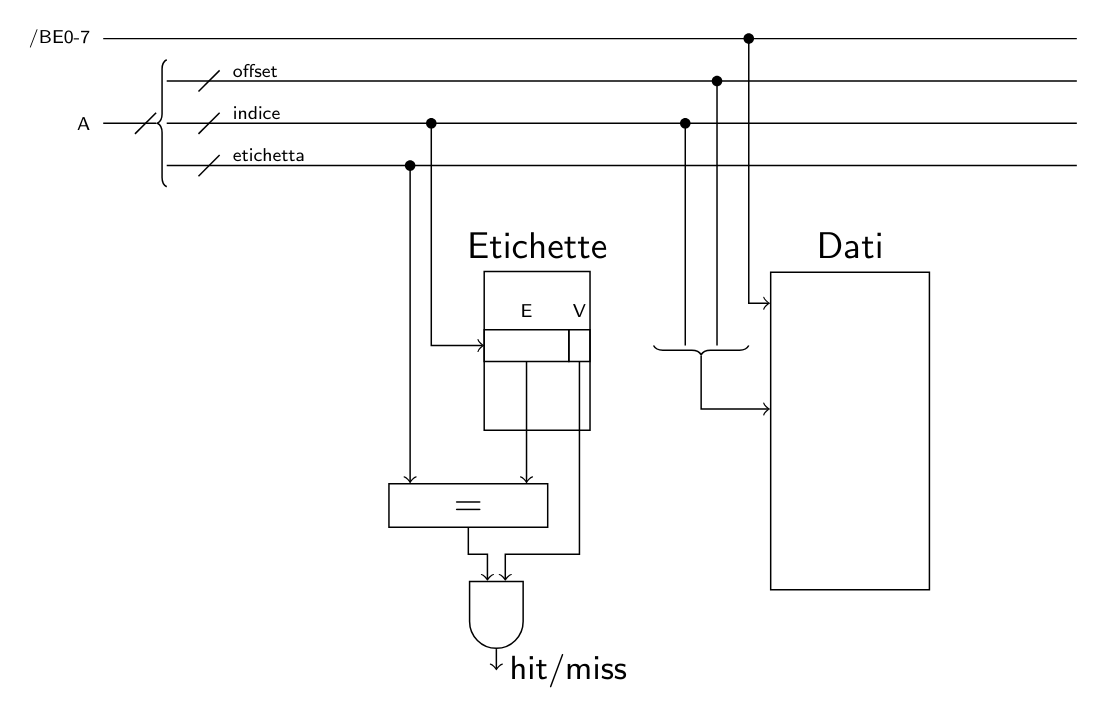
\includegraphics[scale = 0.5]{../figures/cache_diretta.png}
\end{center}

\subsubsection{Lettura}
A questo punto, in fase di lettura, nel caso di hit basterà ricavare una linea di offset dai bit meno significativi di A, e leggere dalla memoria cache a tale offset, all'indice indicato dall'etichetta.
Nel caso di miss si dovrà invece svolgere la lettura in memoria RAM, e poi riportare l'informazione nella cacheline di indice giusto della cache aggiornando l'etichetta.

\subsubsection{Scrittura}
Per quanto riguarda le scritture invece, potremo muoverci in due strade: \textbf{write allocate} e \textbf{write no allocate}.

\begin{itemize}
	\item \textbf{Write allocate:}
ci comportiamo in maniera simile alla lettura nel caso di hit.
Nel caso di miss, invece, riportiamo il dato in cache.

A questo punto potremmo pensare di svolgere la scrittura in RAM e in cache contemporaneamente (regola \textit{write-through}), mantenendo entrambe aggiornate.

Una tecnica più intelligente può invece essere quella di aggiornare il solo dato in cache, e rimandare la scrittura in RAM alla rimozione del dato dalla cache (per l'introduzione di un nuovo dato allo stesso indice) (regola \textit{write-back}).
In questo caso dovremo dotarci di un nuovo bit nella memoria delle etichette, il bit \textit{dirty}, che segnalerà il bisogno di ricopiare il dato in cache nella RAM in occasione del suo deallocamento dalla cache.
La difficoltà principale di questo metodo è l'avere un agente che non è la CPU che scrive in RAM, e come vedremo richiede soluzioni tecniche particolari.

\item \textbf{Write no allocate:}
in questo caso ignoriamo le scritture in cache e la sfruttiamo solamente per le letture.

\end{itemize}

\par\smallskip

Notiamo che questa cache soffre di problemi di \textbf{collisione}: infatti ci sarà un numero di regioni con lo stesso indice ed etichetta diversa, pari alla dimensione della RAM fratto la dimensione della cache.

\end{document}
